\documentclass[a4paper,12pt]{article}
\usepackage[utf8]{inputenc}
\usepackage[czech]{babel}
\usepackage{graphicx}
\usepackage{hyperref}
\usepackage{placeins}
\usepackage{pdflscape}
\emergencystretch=2em

\title{
    Interpret jazyka SOL26 \\[1ex]
    \large Dokumentace k projektu IPP
}
\author{
    Radim Pokorný (xpokorr00)
}
\date{\today}

\begin{document}

\begin{titlepage}
    \begin{center}
        % ---- LOGO FIT VUT ----
        
\includegraphics[width=0.6\textwidth]{FIT_VUT_logo.png}\\[2cm]
        
        % ---- TITULEK ----
        {\LARGE \textbf{Interpret jazyka SOL26}}\\[1ex]
        {\large Dokumentace k projektu IPP}\\[3cm]
        {\large Varianta -- {PHP, Python}}\\[3cm]
        
        % ---- AUTOR ----
        \textbf{Radim Pokorný (xpokorr00)}
        
        \today
    \end{center}
\end{titlepage}

\tableofcontents
\newpage

\section{Úvod}
Tato dokumentace popisuje stručné specifikace implementace interpretu pro jazyk SOL26, pro který již byl vytvořen parser ve formátu 
XML. Cílem tohoto projektu je dodržet předem dané specifikace OO návrhu.

\section{Návrh}
Systém interpretu pracuje ve třech fázích. Nejprve validuje vstup, poté provede sémantickou analýzu a nakonec vykoná program.
Nejprve se rozebere XML strom, který je validován pomocí knihovny \texttt{pydantic-xml}. První kontrola je tedy provedena. 
Dále se provádí sémantická analýza, která ověřuje, zda je přítomna třída \texttt{Main} a hlavní metoda \texttt{run}.
Kontroluje se také arita metod, kde je nutné splňovat pravidlo počtu dvojteček v selektoru s počty parametrů.
Jakmile je provedena sémantická analýza, je buďto vrácen určený chybový stav nebo se přejde na rekurziní vykonání programu,
který využívá datovou strukturu \texttt{Environment}.

Celková architektura je řešena modulárně, kde se syntaktická validace, sémantická analýza a běh programu provadí na různých místech.
Během návrhu byl kladen důraz i na přehlednost a využití tříd pro jednotlivé datové struktury, které jsou zmíněny v příští kapitole.

Po dokončení sestavení syntaktického stromu následuje fáze sémantické analýzy, kde interpret prochází deklarace všech objektů a metod.
Tyto objekty jsou průběžně ukládány do slovníků, avšak prvním pravidlem je vždy ověření existence objektu \texttt{Main} a jeho metody \texttt{run}.
Dále se provádí kontrola arity metod, přičemž v jazyce \texttt{SOL26} je přítmnost znaku \texttt{:} poměrně velká obtíž, která si žádá důslednou režii.

Základem vykonávání programu je prochází syntaktického stromu rekurzivně. Během průchodu dochází k zasílání zpráv mezi objekty, kde se vykonávají instrukce.
U nich musí být vždy jasné kdo je odesílá a její příjemce. Dále hledá implementaci vykonávané metody pomocí metody \texttt{lookup}, kde se směrem k rodiči postupně snaží dostat
ke svému cíli, což umožňuje použití dědičnosti a polymorfismu.

Aby byl zachován správně rozsah platnosti, je využita implementovaná třída \texttt{Environment}. Každé volání metody a deklarace bloku vytváří novou instanci této třídy.
Tato třída zajištujě obecný přehled a je jedním z nejdůležitějších stavebních kamenů implementace.


\begin{figure}[ht!]
    \centering
    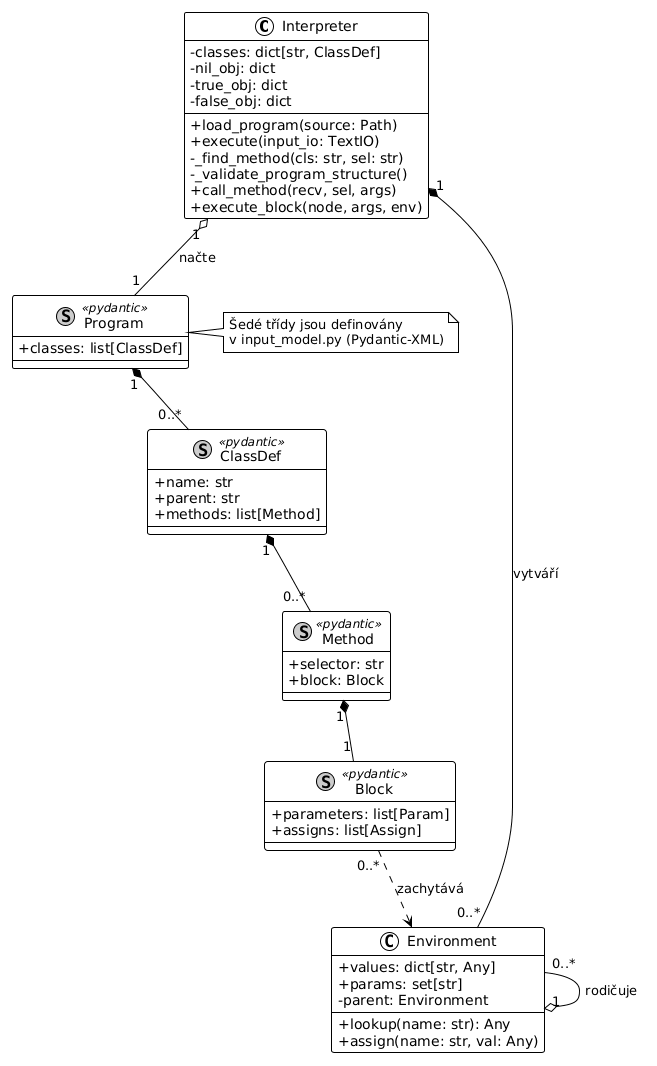
\includegraphics[width=1.0\textwidth]{int_class.png}
    \caption{UML diagram tříd interpretu SOL26}
    \label{fig:class_diagram}
\end{figure}
\FloatBarrier

\section{Datové struktury}
\texttt{Environment} je datová struktura, která uchovává paměťový rámec na rozsah platnosti proměnných. Obsahuje slovník
hodnot a odkazuje na nadřazené prostředí téhož typu, tedy na svého rodiče. Díky této funkcionalitě umožňuje lexikální vyhledávání 
a uzávěry.

\texttt{Interpreter} je sice již převzatá datová struktura, ale byla doplněna o kompletní logiku životního cyklu programu.
Používá metody pro vyhodnocování výrazů \texttt{evaluate\_expr} a správu lokálních rozsahů v \texttt{execute\_block}, kde využívá třídu
\texttt{Environment}. 

Veškeré objekty jsou v implementaci reprezentovány v datovém typu slovník, kde jsou uloženy názvy tříd, atributy i hodnoty.

\section{Využití návrhových vzorů a principů OOP}
Architektura projektu využívá OO paradigma pro lepší dekompozici složitějších problémů a jednodušší spolupráci entit.
Místo procedurálního zpracování instrukcí je kladen důraz na zapouzdření do logických celků a definice rozhraní komponent.

\subsection{Command a Message Dispatching}
Tento vzor je v implementaci naprosto klíčový a jeho jádro je umístěno v metodě \texttt{call\_method}.
Interpret při každém volání zasílá zprávu svému příjemci, tedy objektu, kde pak na základě selektoru dohledá logiku v
odpovídající třídě nebo tabulkách. Díky tomuto přístupu lze interpret v budoucnu rozšířit bez komplikací a nutnosti zasahovat přímo
do implementace logiky.

\subsection{Řetězec zodpovědnosti}
Tento princip je schopen fungovat díky implementaci datové strukury \texttt{Environment}. Jakékoliv prostředí drží odkaz na svého
rodiče a díky tomuto vzniká koncept lineární hierarchie, kde se požadavky typu \texttt{assign} nebo třeba \texttt{lookup} zpropagují
nahoru, dokud se v příslušném prostředí nenalezne hledaný identifikátor. Tento princip je pro implementaci a optimalizaci velmi vhodný
vzhledem k tomu, že by šlo ještě použít globální tabulku symbolů, což by bylo mnohem méně vhodné.

\subsection{Singleton a Immutable Objects}
Ve tříde \texttt{Interpreter} jsou vytvořeny instance objektů \texttt{nil, true} a \texttt{false} pouze jednou a jsou 
uloženy do atributů \texttt{nil\_obj, true\_obj} a \texttt{false\_obj}. Všechny komponenty pak odkazují na tyto instance, což
v jazyce Python hodně urychluje porovnání operátorem \texttt{is}. Díky tomuto vzoru se interpret chová konzistentně a zaručuje
správnost logických operací kdekoliv v programu.

\section{Problémy a výzvy během implementace}
Během implementace interpretu bylo třeba pochopit více do hloubky jazyk Python a také přesně definovat typy
proměnných v kódu, což přinášelo mnoho problémů. Dále některé koncepty OOP, na které byl brán větší ohled 
až v~ne úplně rané fázi programování, způsobily mnoho komplexních výzev.

\subsection{Problém s logickými hodnotami}
Během testování interpretu jednotlivými programy došlo na vyhodnocení výrazu \texttt{false == false}, kde se jako výsledek očekává
rovnost, ale výsledkem po několika pokusech byl stále \texttt{false}. Příčinou bylo, že interpret při každém výskytu literálu
vytvořil nový slovník reprezentující objekt. Zadání vyžaduje, aby se porovnávala identita, nikoliv vnitřní hodnoty.
Problém byl vyřešen zavedením statických objektů \texttt{self.true\_obj, self.false\_obj} a \texttt{self.nil\_obj} v inicializaci interpretu.
Poté, když se provadí jakékoliv porovnání, tak se porovnávají tyto jedinečné instance objektů.

\subsection{Kolize názvů metod a atributů}
Při definici stejným názvem např. getteru a metody si program nedokázal poradit s jejich odlišností a vracel automaticky
hodnotu atributu u getteru. Docházelo tedy k nepředvídatelnému chování v rámci dědičnosti. 
Řešením bylo přidání kontroly do metody \texttt{\_handle\_attribute\_access}. 
Pokud se interpret pokusí přistoupit k atributu, 
nejprve pomocí \texttt{\_find\_method} ověří, zda v hierarchii tříd neexistuje metoda se stejným selektorem.
Jestliže k tomu dojde, vrátí se sémantická chyba.

\subsection{Rekurzivní hloubka a uzávěry}
Při vykonání cyklů typu \texttt{whileTrue:} docházelo k chybnému hledání promeněných, kde byl problém u bloků.
Bloky v cyklu ztrácely kontakt s třídou \texttt{Environment}. Blok v implementaci nesmí být vykonáván v prostředí 
svého volajícího, ale ve svém nadřazeném. Řešení bylo nakonec triviální, ale těžké k nalezení. 
Stačilo danému bloku přidat referenci na aktuální \texttt{Environment}.

\section{Zamyšlení nad možnostmi dalšího rozšíření}
Byly vybrány 3 rozšíření, které by šli hladce implementovat vzhledem k již uvedeném návrhu.

\subsection{Třídy jako objekty první kategorie}
Toto rozšíření by šlo teoreticky implementovat, jelikož v kódu se důmyslně rozlišují statické a instanční metody ve funkci \texttt{\_handle\_static\_methods}.
Ve slovníku \texttt{self.classes} by se prvky retransformovali na objekty instance metatřídy \texttt{Class}. Její metody by mohly být uloženy v samostatné
tabulce metod, kde by vyhledávání spočívalo ve sdílení instančních metod po pár úpravách metody \texttt{\_find\_method}.

\subsection{Modifikátory přístupu}
V interpretu se výrazy vyhodnocují rekurzivně v metodě \texttt{evaluate\_expr}, která do následně volané metody \texttt{call\_method} 
již předává parametr \texttt{defining\_class}. Tento parametr reprezentuje třídu, ve které je volání prováděno, 
a definuje tak kontext odesílatele zprávy.
Při vyhledávání metody v mechanismu \texttt{lookup} by se nově kontrolovala viditelnost. Logika by porovnala kontext v \texttt{defining\_class} s třídou, 
kde byla metoda nalezena. Pomocí existující metody \texttt{\_is\_subclass} by se ověřilo, 
zda je odesílatel v hierarchii dědičnosti oprávněn k přístupu.
Pokud by podmínky nebyly splněny, interpret by vyvolal chybu nenalezení metody. Celkově by tedy nebylo nutné měnit architekturu, 
pouze doplnit logiku do lookup mechanismu.

\subsection{Mechanismus \texttt{doesNotUnderstand}}
V návrhu \texttt{call\_method} by bylo toto rozšíření poměrně triviální záležitost. V podstatě místo výjimky \texttt{InterpreterError} v této metodě by
se vytvořila instance třídy \texttt{Message}, která by obsahovala vnitřní stav \texttt{val} původního selektoru a zbytek jeho argumentů.
Díky návrhu interpretu, kde se veškerý \texttt{Dispatching} odehrává na jednom místě, není třeba zasahovat do implementace vyhodnocení výrazů a celkově
sémantických kontrol.

\section{Využití generativní umělé inteligence}
Během implementace, zprovoznění projektu, návrhu Dockerfile apod. byly použity jazykové modely \texttt{ChatGPT} a \texttt{Gemini}.
Pomohli mi také objasnit mé zkušenosti s OOP ze střední školy, které jsem si musel znovu připomenout a trochu obohatit.
Dále mi byla velmi nápomocna při vysvětlení návrhových vzorů a pokročilejších úvah, kdy jsem potom měl lepší představu o implementaci.
Konverzace s umělou inteligencí jsou přiloženy odkazem v souboru \texttt{ai-chatgpt.md} a \texttt{ai-gemini.md}.

\section{Změny po prvním odevzdání}
V automatizovaných testech nešly spustit binární soubory pro kontrolu kvality kódu. Do Dockerfile byl 
přidán jeden řádek, který přidává \texttt{symlinks} a~ostatní potřebné nástroje pro zajištění bezproblémového běhu.

\end{document}